\subsection{Predictive Performance Across Datasets (RQ1)}

Table~\ref{tab:cv_model_results} summarizes the five-fold cross-validation
performance of AdaBoost, XGBoost, and LightGBM on the three healthcare
datasets. The values are reported as mean $\pm$ standard deviation across the
five validation folds. PR-AUC is treated as the primary comparison metric,
while ROC-AUC, Recall, and F1-score provide complementary views of ranking and
threshold-based performance.

\begin{table}[H]
\centering
\begin{minipage}{0.90\linewidth}
\centering
    \refstepcounter{table}
    \begin{captionbelowboxaivn}
        \captable{Five-fold cross-validation performance (mean $\pm$ standard deviation).}
        \label{tab:cv_model_results}
    \end{captionbelowboxaivn}

    \renewcommand{\arraystretch}{1.1}
    \small

    \begin{tabularx}{\linewidth}{@{}
        >{\raggedright\arraybackslash}X
        >{\raggedright\arraybackslash}X
        >{\centering\arraybackslash}X
        >{\centering\arraybackslash}X
        >{\centering\arraybackslash}X
        >{\centering\arraybackslash}X@{}}
	\textbf{Dataset} & \textbf{Model} & \textbf{ROC-AUC} & \textbf{PR-AUC} & \textbf{Recall} & \textbf{F1} \\
\hline
Dataset 1 & AdaBoost & $0.8715 \pm 0.0042$ & $0.3853 \pm 0.0087$ & $0.6794 \pm 0.0106$ & $0.3765 \pm 0.0082$ \\
 & XGBoost & $0.8873 \pm 0.0031$ & $0.4138 \pm 0.0092$ & $0.7799 \pm 0.0071$ & $0.3328 \pm 0.0023$ \\
 & LightGBM & $0.8871 \pm 0.0034$ & $0.4127 \pm 0.0090$ & $0.7760 \pm 0.0097$ & $0.3347 \pm 0.0029$ \\
\hline
Dataset 2 & AdaBoost & $0.9240 \pm 0.0429$ & $0.9228 \pm 0.0438$ & $0.8449 \pm 0.0294$ & $0.8587 \pm 0.0169$ \\
 & XGBoost & $0.9274 \pm 0.0332$ & $0.9248 \pm 0.0338$ & $0.8794 \pm 0.0451$ & $0.8780 \pm 0.0234$ \\
 & LightGBM & $0.9249 \pm 0.0303$ & $0.9169 \pm 0.0329$ & $0.8818 \pm 0.0235$ & $0.8787 \pm 0.0169$ \\
\hline
Dataset 3 & AdaBoost & $0.8324 \pm 0.0031$ & $0.3678 \pm 0.0078$ & $0.7727 \pm 0.0082$ & $0.3826 \pm 0.0030$ \\
 & XGBoost & $0.8386 \pm 0.0026$ & $0.3803 \pm 0.0050$ & $0.8014 \pm 0.0075$ & $0.3805 \pm 0.0022$ \\
 & LightGBM & $0.8378 \pm 0.0023$ & $0.3797 \pm 0.0059$ & $0.7955 \pm 0.0047$ & $0.3822 \pm 0.0021$ \\
        \end{tabularx}
\end{minipage}
\end{table}

On Dataset 1, XGBoost and LightGBM produced almost identical ROC-AUC, while
XGBoost achieved a slightly higher mean PR-AUC and Recall. Both gradient-
boosted models clearly exceeded AdaBoost on ROC-AUC, PR-AUC, and Recall. The
lower F1 scores of XGBoost and LightGBM indicate that their higher recall at the
fixed 0.50 threshold came with a precision trade-off.

On Dataset 2, all three models achieved strong discrimination, with mean
ROC-AUC values close to 0.924. XGBoost achieved the highest mean Recall and F1,
whereas AdaBoost obtained the highest mean PR-AUC by a small margin. This shows
that no single model dominated every metric on this relatively small dataset.

On Dataset 3, XGBoost and LightGBM again improved ROC-AUC and PR-AUC over
AdaBoost. XGBoost achieved the highest mean Recall, while the three models had
very similar F1 values. Across the three datasets, the aggregated comparison
ranked XGBoost first with a mean dataset rank of 1.0000, followed by LightGBM at
2.3333 and AdaBoost at 2.6667. XGBoost also achieved the highest cross-dataset
mean ROC-AUC (0.8844), PR-AUC (0.5730), and Recall (0.8202). AdaBoost achieved
the highest cross-dataset mean F1 (0.5392), emphasizing that the preferred model
depends partly on the evaluation objective and decision threshold.

\begin{table}[H]
\centering
\begin{minipage}{0.90\linewidth}
\centering
    \refstepcounter{table}
    \begin{captionbelowboxaivn}
        \captable{Unweighted cross-dataset comparison based on the experiment outputs.}
        \label{tab:overall_model_results}
    \end{captionbelowboxaivn}

    \renewcommand{\arraystretch}{1.1}
    \small

    \begin{tabularx}{\linewidth}{@{}
        >{\raggedright\arraybackslash}X
        >{\centering\arraybackslash}X
        >{\centering\arraybackslash}X
        >{\centering\arraybackslash}X
        >{\centering\arraybackslash}X
        >{\centering\arraybackslash}X@{}}
\textbf{Model} & \textbf{Mean Rank} & \textbf{ROC-AUC} & \textbf{PR-AUC} & \textbf{Recall} & \textbf{F1} \\
\hline
    XGBoost & \textbf{1.0000} & \textbf{0.8844} & \textbf{0.5730} & \textbf{0.8202} & 0.5305 \\
    LightGBM & 2.3333 & 0.8833 & 0.5698 & 0.8178 & 0.5319 \\
    AdaBoost & 2.6667 & 0.8760 & 0.5586 & 0.7657 & \textbf{0.5392} \\
        \end{tabularx}
\end{minipage}
\end{table}

These results answer RQ1 by showing that XGBoost provides the strongest overall
performance under the selected protocol, although LightGBM is extremely close
on several ranking metrics and AdaBoost retains a small advantage in aggregate
F1. Therefore, the comparison does not support a claim that one algorithm is
uniformly superior on every metric and dataset.

\begin{figure}[H]
    \centering
    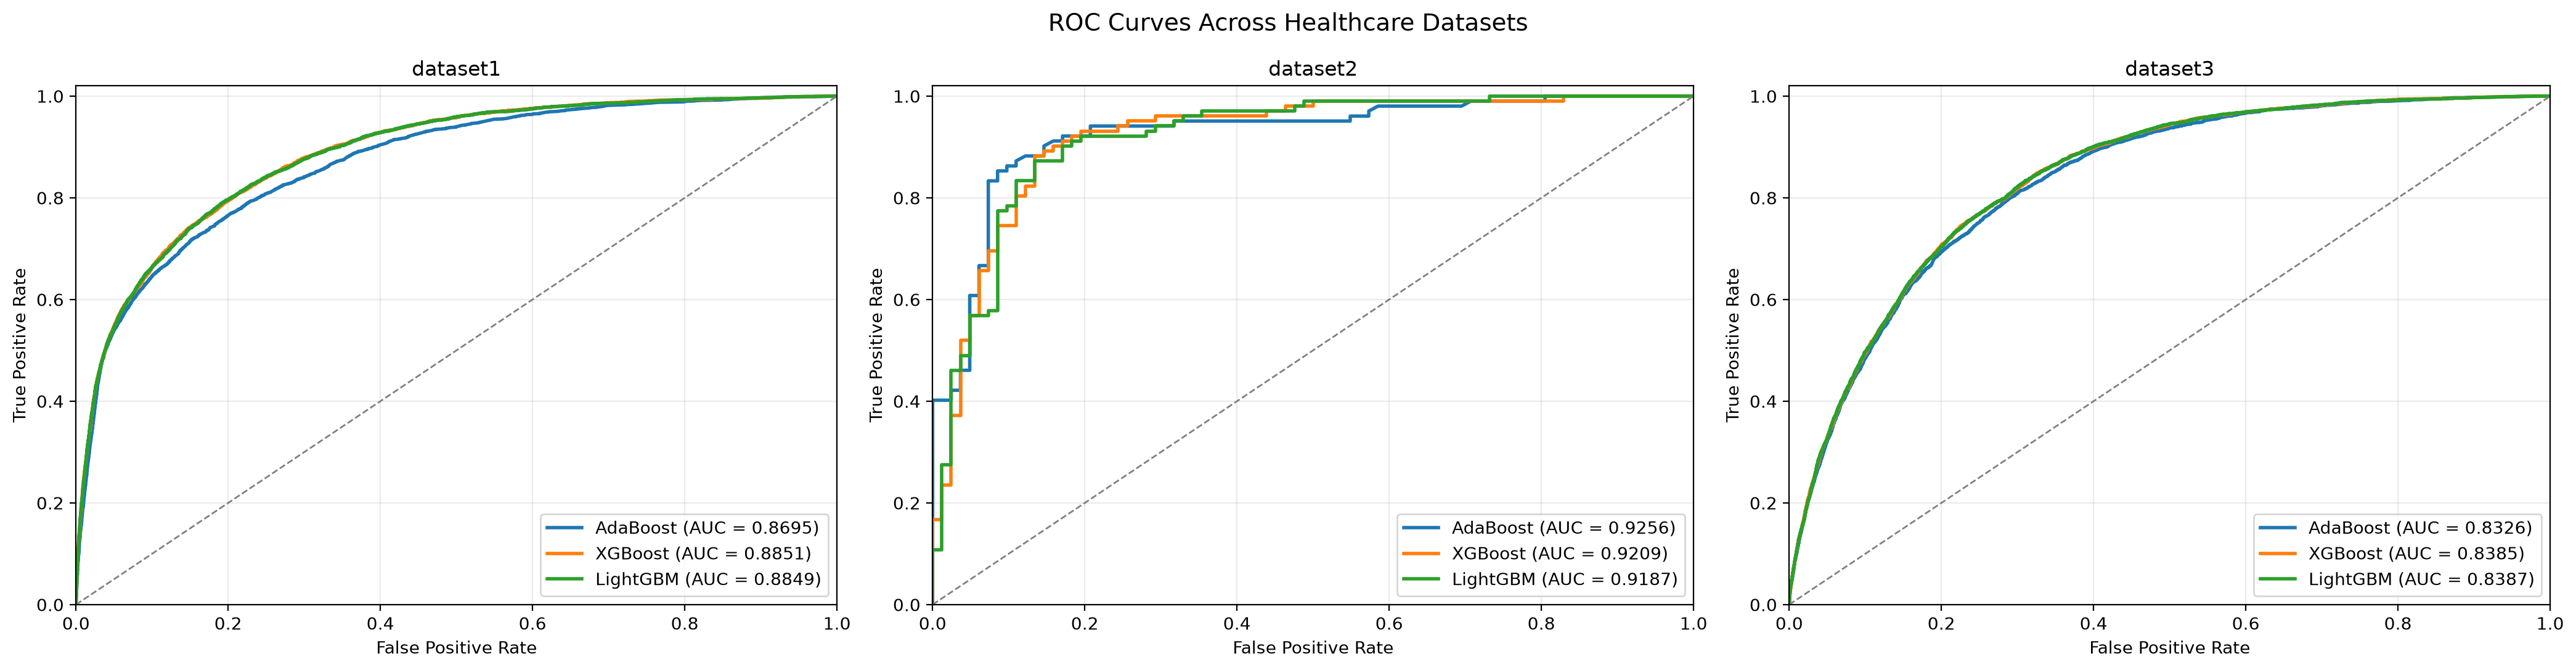
\includegraphics[width=0.95\linewidth]{Figures/roc_curves_all_datasets.png}
    \begin{minipage}{0.95\linewidth}
        \begin{figurecaptionmodern}
        \centering
        \capfig{ROC curves for the three models on the untouched hold-out test sets across the three healthcare datasets.}
        \label{fig:roc-all-datasets}
        \end{figurecaptionmodern}
    \end{minipage}
\end{figure}

The ROC visualization is consistent with the tabulated test results. The curves
are close on Dataset 1 and Dataset 3, where XGBoost and LightGBM provide similar
ranking performance. Dataset 2 has the highest test AUC values overall, but its
step-shaped curves also reflect the smaller test sample and therefore should not
be interpreted as evidence of uniformly better clinical performance across
datasets. The figure supports comparing ranking behavior within each dataset,
not pooling patients from different prediction tasks.

\begin{table}[H]
\centering
\begin{minipage}{0.90\linewidth}
\centering
    \refstepcounter{table}
    \begin{captionbelowboxaivn}
        \captable{Performance on the untouched hold-out test partitions after refitting on the full development data.}
        \label{tab:holdout_model_results}
    \end{captionbelowboxaivn}

        $\rho=0.9324$ but Kendall $\tau=0.7990$. Both values indicate positive and
    \small

    \begin{tabularx}{\linewidth}{@{}
        >{\raggedright\arraybackslash}X
        >{\raggedright\arraybackslash}X
        >{\centering\arraybackslash}X
        >{\centering\arraybackslash}X
        >{\centering\arraybackslash}X
        >{\centering\arraybackslash}X@{}}
\textbf{Dataset} & \textbf{Model} & \textbf{ROC-AUC} & \textbf{PR-AUC} & \textbf{Recall} & \textbf{F1} \\
\hline
Dataset 1 & AdaBoost & 0.8695 & 0.3860 & 0.6705 & 0.3657 \\
 & XGBoost & 0.8850 & 0.4169 & 0.7712 & 0.3255 \\
 & LightGBM & 0.8850 & 0.4187 & 0.7694 & 0.3259 \\
\hline
Dataset 2 & AdaBoost & 0.9256 & 0.9394 & 0.8529 & 0.8832 \\
 & XGBoost & 0.9224 & 0.9216 & 0.8333 & 0.8586 \\
 & LightGBM & 0.9189 & 0.9166 & 0.8431 & 0.8643 \\
\hline
Dataset 3 & AdaBoost & 0.8326 & 0.3672 & 0.7674 & 0.3788 \\
 & XGBoost & 0.8384 & 0.3756 & 0.7963 & 0.3773 \\
 & LightGBM & 0.8385 & 0.3763 & 0.7925 & 0.3789 \\
        \end{tabularx}
\end{minipage}
\end{table}

\subsection{Predictive Stability Across Cross-Validation Folds (RQ2)}

The fold-level results also reveal clear differences in stability across the
three datasets. Dataset 1 and Dataset 3 produced small standard deviations for
all three models. For example, XGBoost obtained ROC-AUC standard deviations of
0.0033 on Dataset 1 and 0.0027 on Dataset 3. LightGBM showed similarly small
variation, indicating that the two gradient-boosted models were not highly
sensitive to the particular fold assignment on the two larger datasets.

Dataset 2 exhibited noticeably greater fold-to-fold variation. Its development
partition contains only 734 samples, compared with 353,653 for Dataset 1 and
183,824 for Dataset 3. XGBoost ROC-AUC ranged from 0.8676 to 0.9465 across the
five folds, while AdaBoost ranged from 0.8547 to 0.9673 and LightGBM ranged from
0.8651 to 0.9497. The larger variability is therefore consistent with the
smaller sample size: each validation fold contains fewer observations, so the
composition of a single fold has a greater influence on the measured score.

The final hold-out results were generally close to the corresponding
cross-validation means. For example, Dataset 1 XGBoost achieved a mean CV
ROC-AUC of 0.8873 and a hold-out ROC-AUC of 0.8851, while Dataset 3 XGBoost
achieved 0.8386 in CV and 0.8385 on the hold-out set. This agreement provides
additional evidence that the reported cross-validation estimates are not driven
by a single unusually favorable split.

Overall, RQ2 is answered by finding that predictive performance is highly stable
on the two large datasets but less stable on the small Heart Failure Prediction
dataset. The pattern is observed across all three algorithms, suggesting that
dataset size and fold composition contribute more to the observed instability
than the choice among the three boosting methods alone.


\subsection{SHAP Feature-Importance Stability Across Cross-Validation Folds (RQ3)}
\label{subsec:shap_results}

Following the fold-wise explainability procedure described in
Section~\ref{subsec:shap_methodology}, RQ3 evaluates whether SHAP-based global
feature-importance rankings remain consistent when the training and validation
partitions change across cross-validation folds. For every dataset--model
combination, all ten unique pairs of the five folds are compared using Kendall's
$\tau$, Spearman's $\rho$, and top-10 Jaccard similarity.

Table~\ref{tab:shap_stability_results} shows that the SHAP feature rankings are
generally stable across folds for all nine dataset--model combinations.
Mean Spearman correlations range from 0.9324 to 0.9921, indicating strong
agreement in the complete feature ordering. Mean Kendall coefficients range
from 0.7990 to 0.9636, providing additional evidence that most pairwise feature
ordering relationships are preserved across folds. Top-10 Jaccard similarity
ranges from 0.7758 to 1.0000, indicating that the most influential feature sets
are also largely consistent.

\begin{table}[H]
\centering
\begin{minipage}{0.90\linewidth}
\centering
    \refstepcounter{table}
    \begin{captionbelowboxaivn}
        \captable{Mean SHAP feature-ranking stability across the ten pairwise comparisons of five cross-validation folds.}
        \label{tab:shap_stability_results}
    \end{captionbelowboxaivn}

    \renewcommand{\arraystretch}{1.1}
    \small

    \begin{tabularx}{\linewidth}{@{}
        >{\raggedright\arraybackslash}X
        >{\raggedright\arraybackslash}X
        >{\centering\arraybackslash}X
        >{\centering\arraybackslash}X
        >{\centering\arraybackslash}X@{}}
\textbf{Dataset} &
\textbf{Model} &
\textbf{Kendall $\tau$} &
\textbf{Spearman $\rho$} &
\textbf{Top-10 Jaccard} \\
\hline
Dataset 1 & AdaBoost & 0.9593 & 0.9644 & 0.9273 \\
          & XGBoost  & 0.7990 & 0.9324 & 0.8273 \\
          & LightGBM & 0.8057 & 0.9368 & 0.7758 \\
\hline
Dataset 2 & AdaBoost & 0.8536 & 0.9410 & 0.8061 \\
          & XGBoost  & 0.8118 & 0.9346 & 0.8545 \\
          & LightGBM & 0.8301 & 0.9422 & 0.8364 \\
\hline
Dataset 3 & AdaBoost & 0.9636 & 0.9921 & \textbf{1.0000} \\
          & XGBoost  & 0.9255 & 0.9814 & \textbf{1.0000} \\
          & LightGBM & 0.8996 & 0.9735 & 0.9273 \\
        \end{tabularx}
\end{minipage}
\end{table}

Dataset 3 demonstrates particularly strong explanation stability. AdaBoost and
XGBoost both obtain a mean top-10 Jaccard score of 1.0000, indicating that the
same set of ten most influential features is retained across every fold pair.
LightGBM achieves the highest overall mean Spearman correlation of 0.9735,
showing that its complete feature ranking is also highly consistent. The high
Kendall coefficients for all three models further confirm that the relative
ordering of feature pairs changes only modestly across partitions.

Dataset 1 also exhibits strong overall stability, although the different
metrics reveal some variation near the top of the ranking. AdaBoost achieves
the strongest agreement on this dataset, with mean Kendall $\tau=0.9593$,
Spearman $\rho=0.9644$, and top-10 Jaccard similarity of 0.9273. LightGBM,
however, obtains a high Spearman correlation of 0.9368 while its top-10 Jaccard
similarity is lower at 0.7758. This result indicates that the complete ranking
remains similar across folds even though several features near the top-10
boundary exchange positions or move into and out of the top feature set.

The difference between the Kendall and Spearman measurements is also
informative. For example, Dataset 1 XGBoost achieves Spearman
$\rho=0.9324$ but Kendall $\tau=0.7990$. Both values indicate positive and
strong ranking agreement, but Kendall's lower value suggests that some
pairwise feature orderings change across folds even though the overall ranking
structure remains similar. Reporting both statistics therefore provides a more
complete view of explanation robustness than relying on a single correlation
measure.

Dataset 2 remains reasonably stable despite being substantially smaller than
Datasets 1 and 3. All three models obtain mean Spearman correlations greater
than 0.93, while mean Kendall coefficients range from 0.8118 to 0.8536.
Top-10 Jaccard similarity ranges from 0.8061 to 0.8545. These values indicate
that the majority of important features remain consistently ranked even though
some movement occurs between folds.

The SHAP beeswarm plots complement the global importance rankings by showing
both the magnitude and direction of feature contributions. Features appearing
near the top of the beeswarm plots have large absolute effects on the model
output, while the horizontal distribution of SHAP values indicates whether
particular feature values tend to increase or decrease the predicted risk.
The corresponding mean absolute SHAP bar plots provide a simpler view of
global importance, and the violin plots show the distribution of SHAP effects
for the leading features.

The feature-ranking heatmaps provide a direct visualization of explanation
stability across folds. Features whose heatmap cells remain at similar rank
values across all five folds can be considered highly stable, whereas large
changes in rank indicate sensitivity to the particular training partition.
This visualization is especially useful for distinguishing small changes near
the top-10 cutoff that may reduce Jaccard similarity without substantially
changing the complete ranking.

The fold-correlation heatmaps provide an additional model-level view of
stability. High off-diagonal Spearman correlations indicate that different
training folds produce similar global feature orderings. A fold with
substantially lower correlations to the other folds would suggest that the
corresponding training partition produces a noticeably different explanation.
Together with the ranking heatmaps, these plots allow the numerical stability
scores to be visually inspected rather than interpreted only from aggregated
statistics.

Overall, RQ3 is answered by finding that SHAP-based global feature-importance
rankings are robust to cross-validation partitioning for the evaluated boosting
models. This conclusion is supported by three complementary measures:
Kendall's $\tau$ shows strong pairwise ordering agreement, Spearman's $\rho$
shows high consistency in complete feature rankings, and top-10 Jaccard
similarity shows that the most influential feature sets are generally
preserved.

At the same time, the results demonstrate why multiple stability metrics are
necessary. A model can maintain a high full-ranking correlation while still
showing changes in the membership of its top-10 features. Consequently,
explanation stability should not be judged from a single correlation
coefficient alone. Combining rank correlations, top-feature overlap,
feature-ranking heatmaps, and fold-correlation heatmaps provides a more
complete assessment of the reproducibility of model explanations.

The observed SHAP stability should be interpreted as evidence of explanation
robustness rather than causal validity. A feature that is consistently
important across folds is repeatedly used by the model under the observed data
distribution, but this does not imply that changing that feature would
causally alter a patient's health outcome. In addition, because AdaBoost uses
permutation SHAP while XGBoost and LightGBM use TreeSHAP, raw SHAP magnitudes
are not used for direct cross-model comparisons. RQ3 therefore focuses on
within-model fold-to-fold ranking stability, which remains comparable across
the experimental protocol.

\begin{figure}[H]
    \centering
    \begin{minipage}{0.32\linewidth}
        \centering
        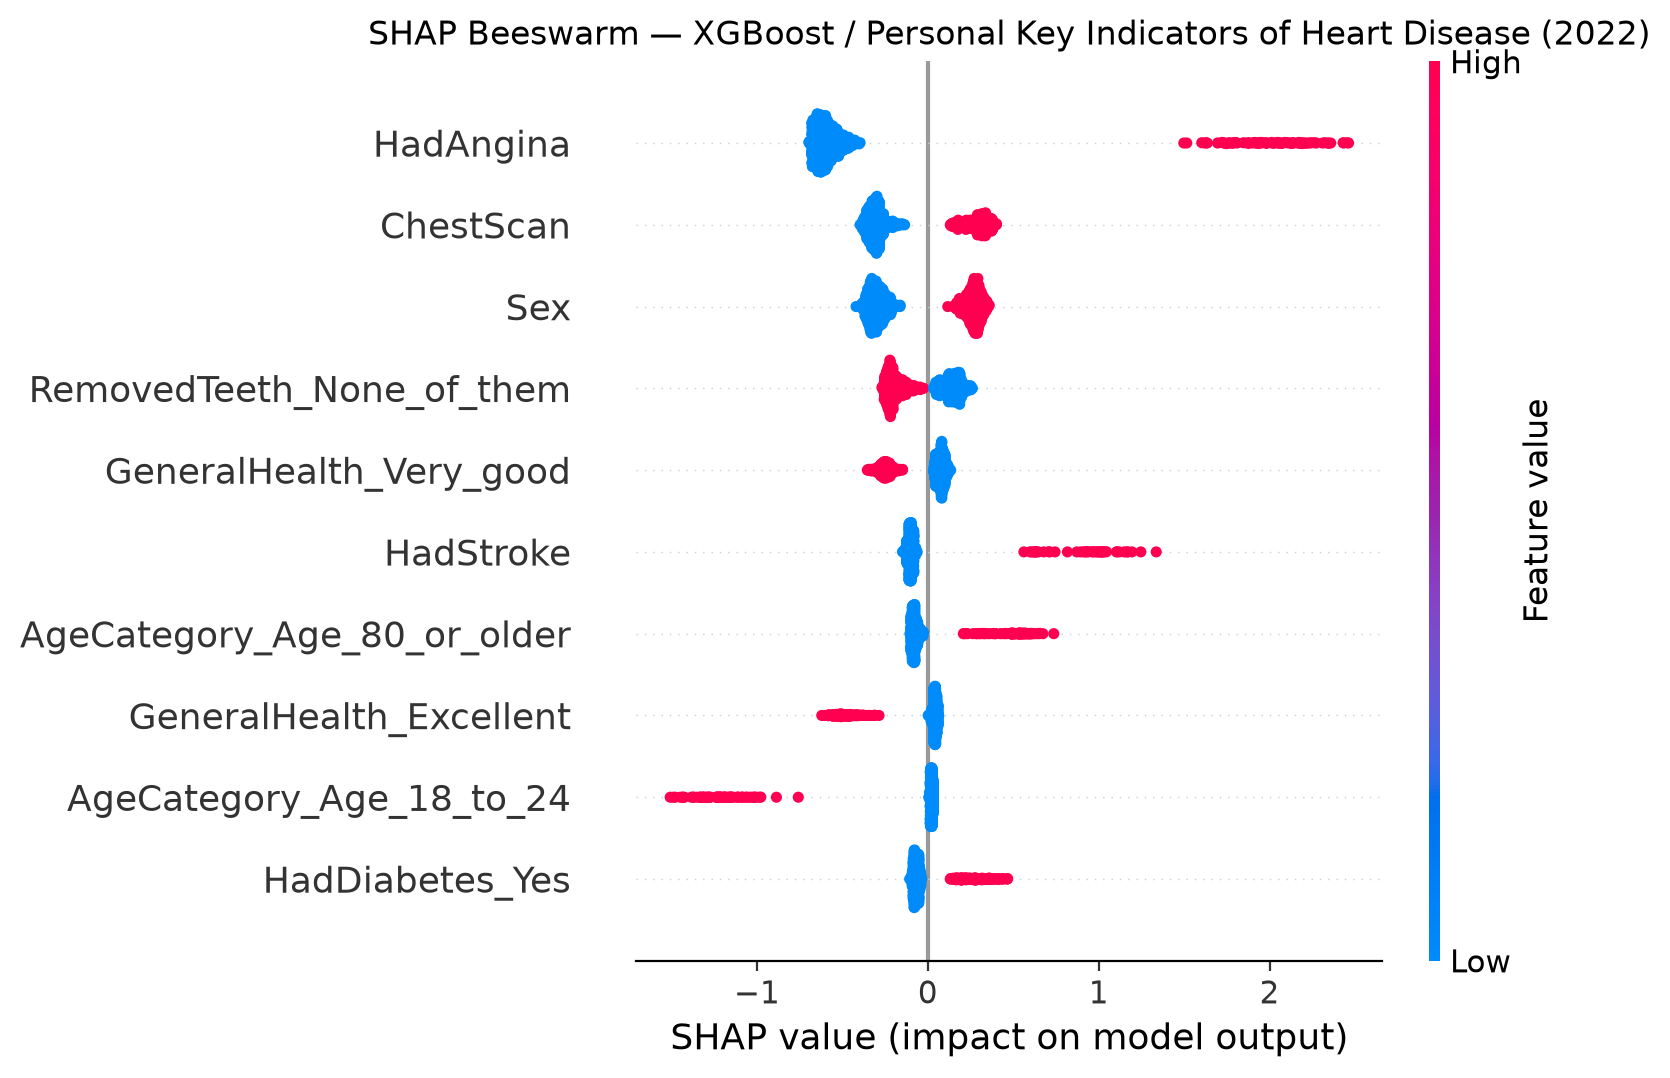
\includegraphics[width=\linewidth]{Figures/dataset1_xgboost_beeswarm.png}
    \end{minipage}\hfill
    \begin{minipage}{0.32\linewidth}
        \centering
        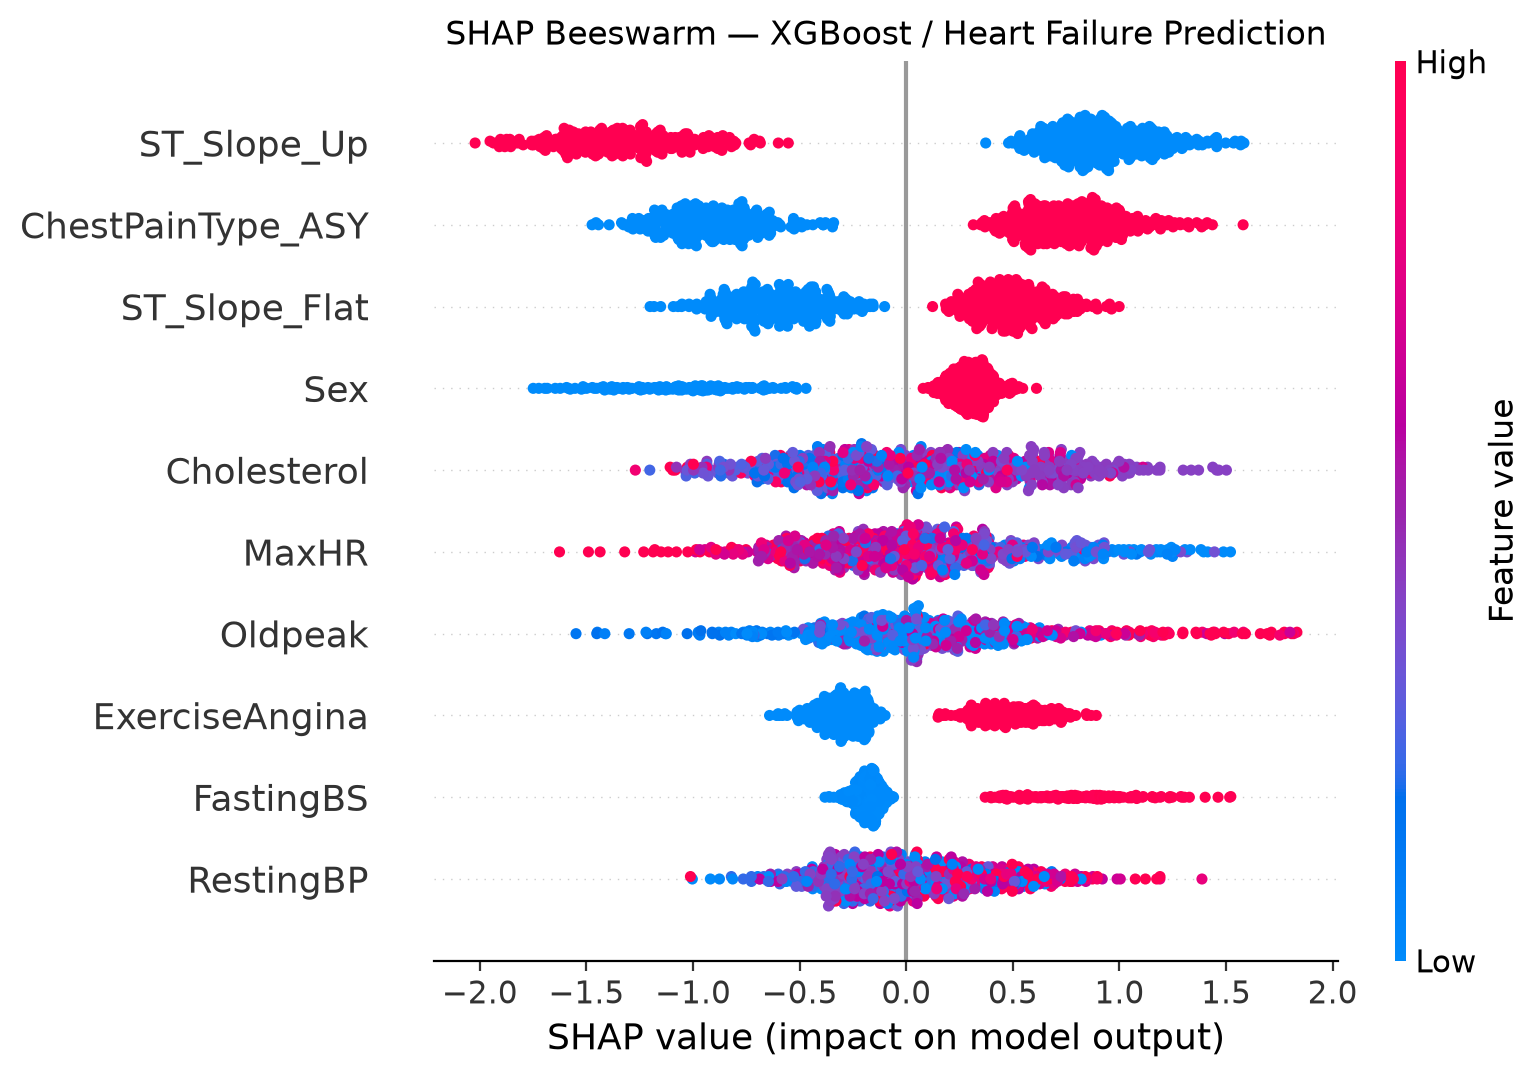
\includegraphics[width=\linewidth]{Figures/dataset2_xgboost_beeswarm.png}
    \end{minipage}\hfill
    \begin{minipage}{0.32\linewidth}
        \centering
        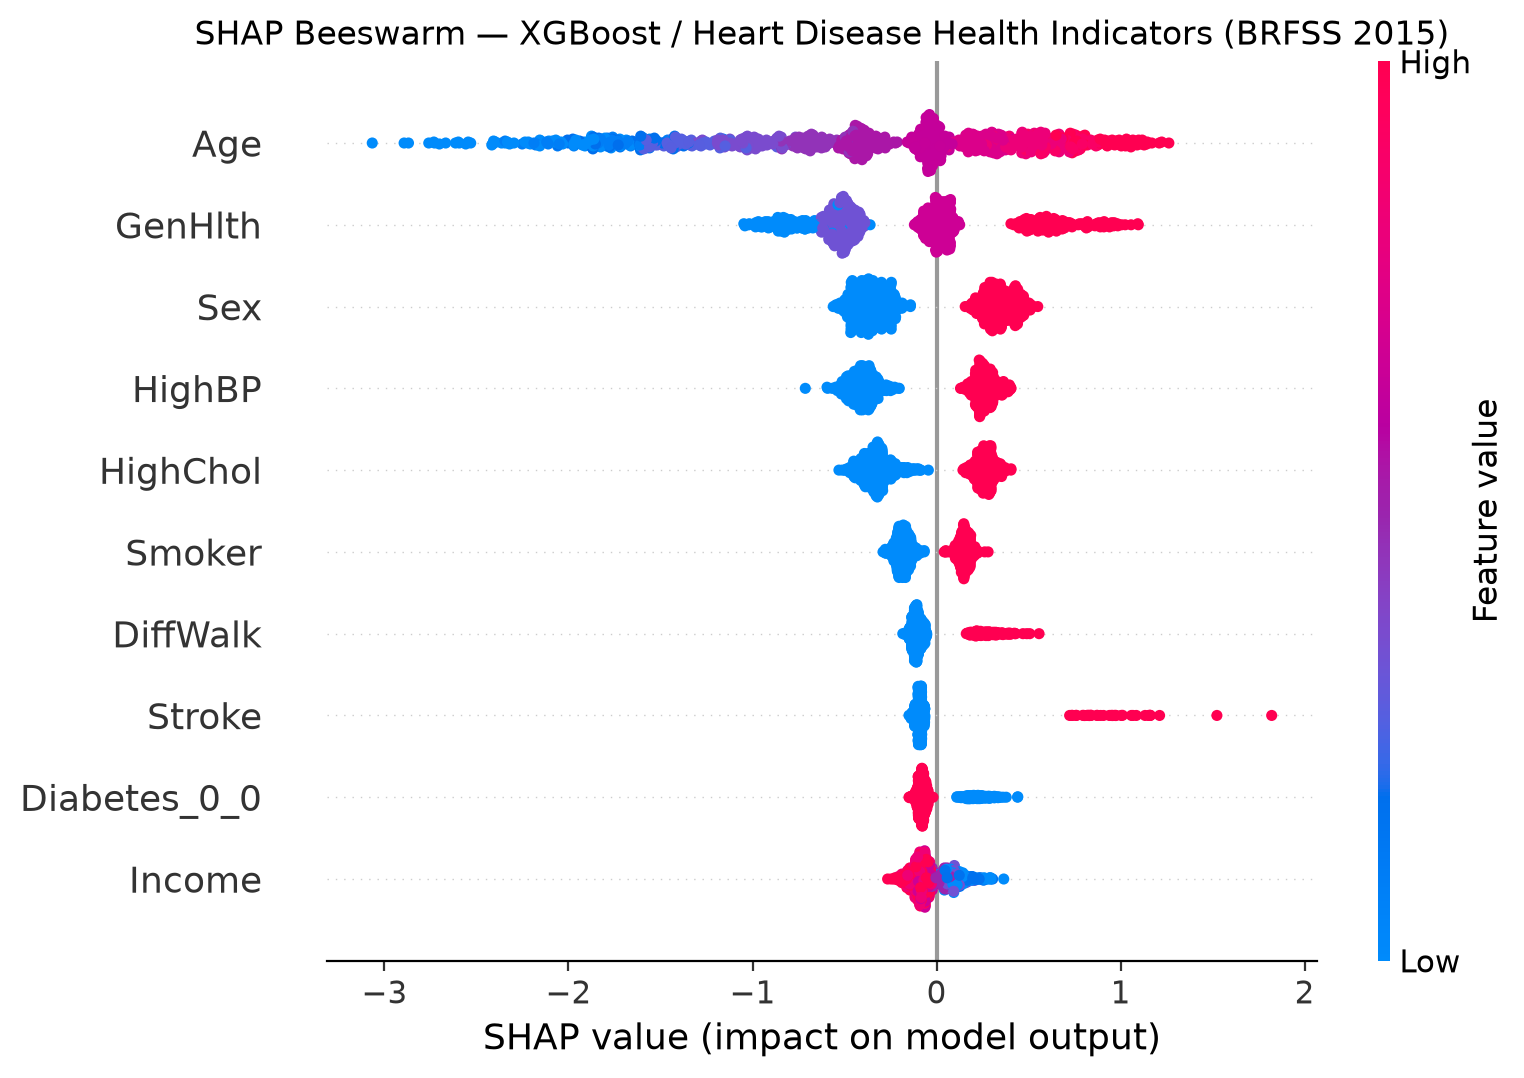
\includegraphics[width=\linewidth]{Figures/dataset3_xgboost_beeswarm.png}
    \end{minipage}
    \begin{minipage}{0.95\linewidth}
        \begin{figurecaptionmodern}
        \centering
        \capfig{SHAP beeswarm plots for XGBoost on Dataset 1, Dataset 2, and Dataset 3, respectively.}
        \label{fig:xgboost-beeswarm-datasets}
        \end{figurecaptionmodern}
    \end{minipage}
\end{figure}

The beeswarm plots show that the most influential features are dataset-specific.
For Dataset 1, \texttt{HadAngina}, \texttt{ChestScan}, and \texttt{Sex} occupy
the leading positions. Dataset 2 is dominated by \texttt{ST\_Slope\_Up},
\texttt{ChestPainType\_ASY}, and \texttt{ST\_Slope\_Flat}, whereas Dataset 3
is led by \texttt{Age}, \texttt{GenHlth}, and \texttt{Sex}. The horizontal
position indicates contribution direction and magnitude, while color encodes
the feature value. These patterns show why a single cross-dataset feature
interpretation would be misleading even when the same model family is used.

\begin{figure}[H]
    \centering
    \begin{minipage}{0.48\linewidth}
        \centering
        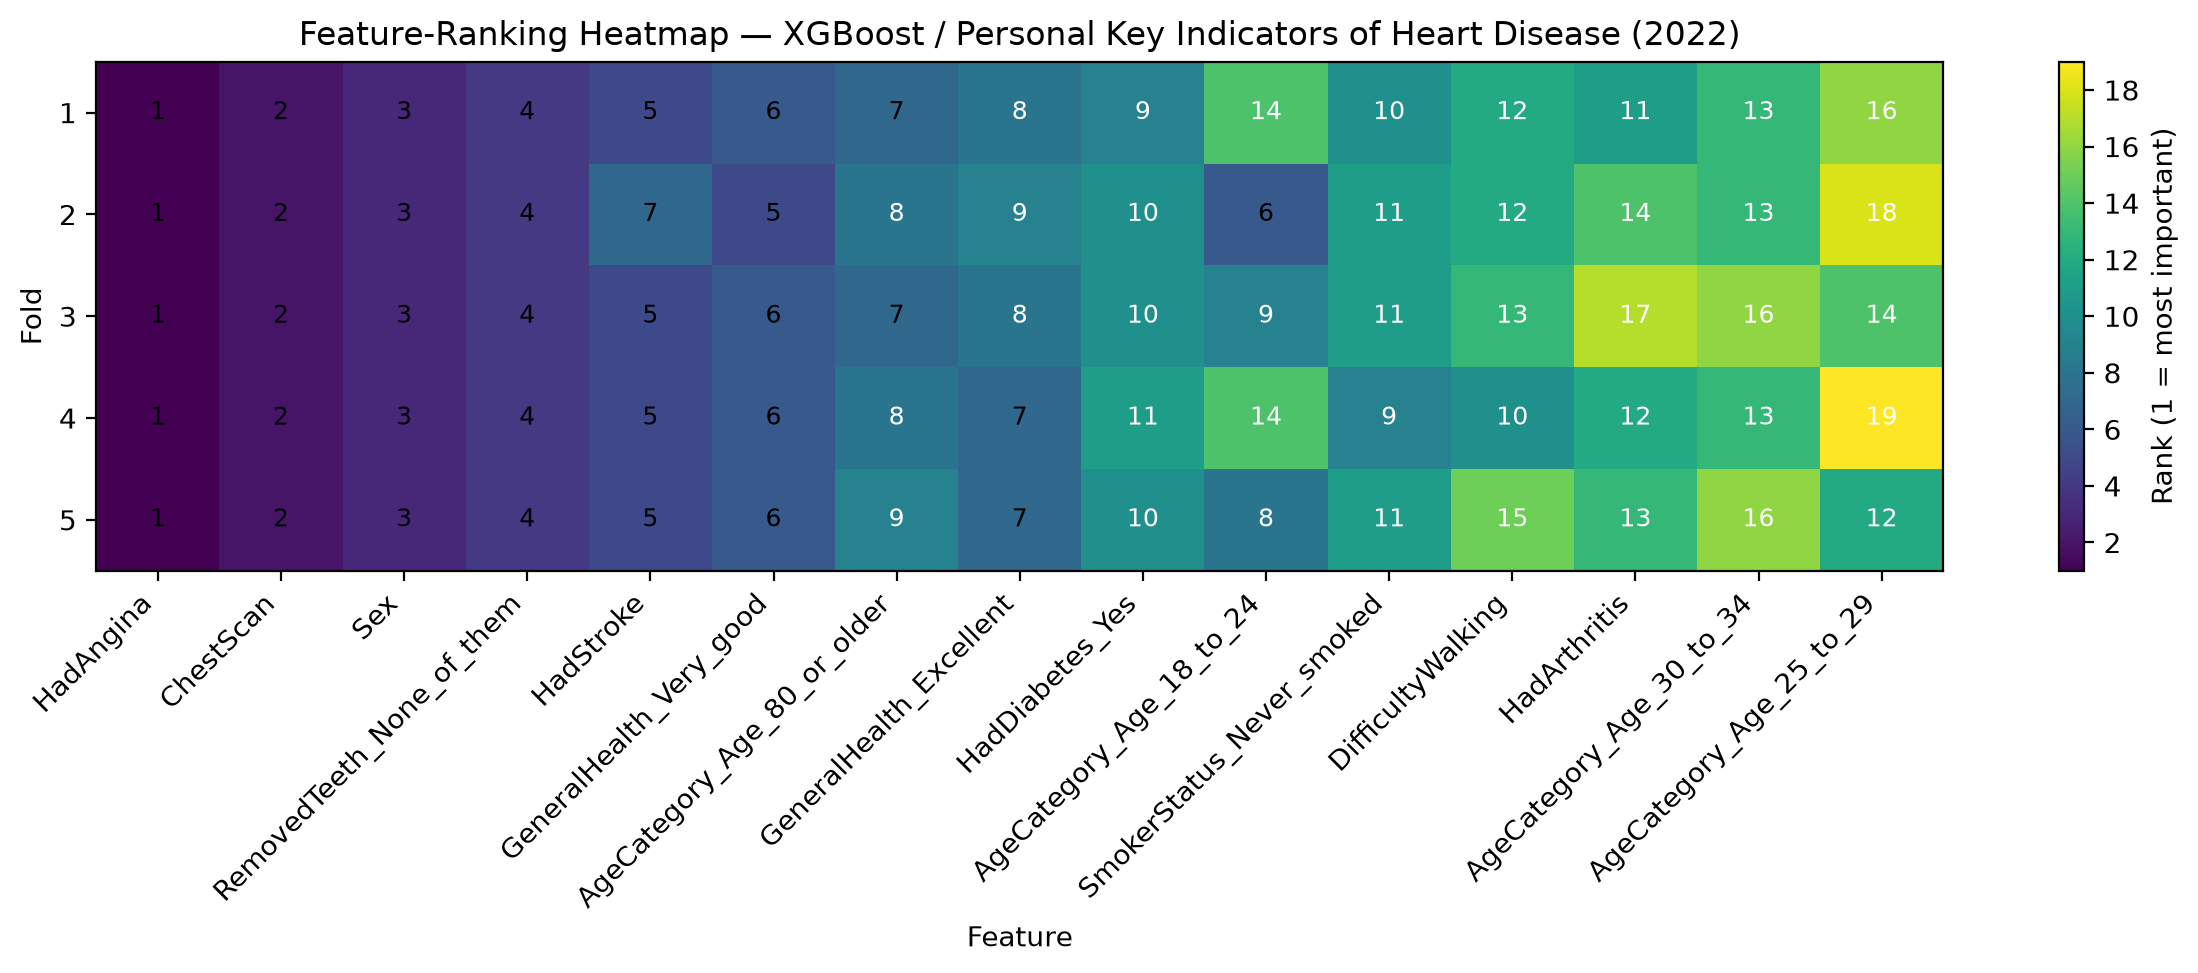
\includegraphics[width=\linewidth]{Figures/dataset1_xgboost_ranking_heatmap.png}
    \end{minipage}\hfill
    \begin{minipage}{0.48\linewidth}
        \centering
        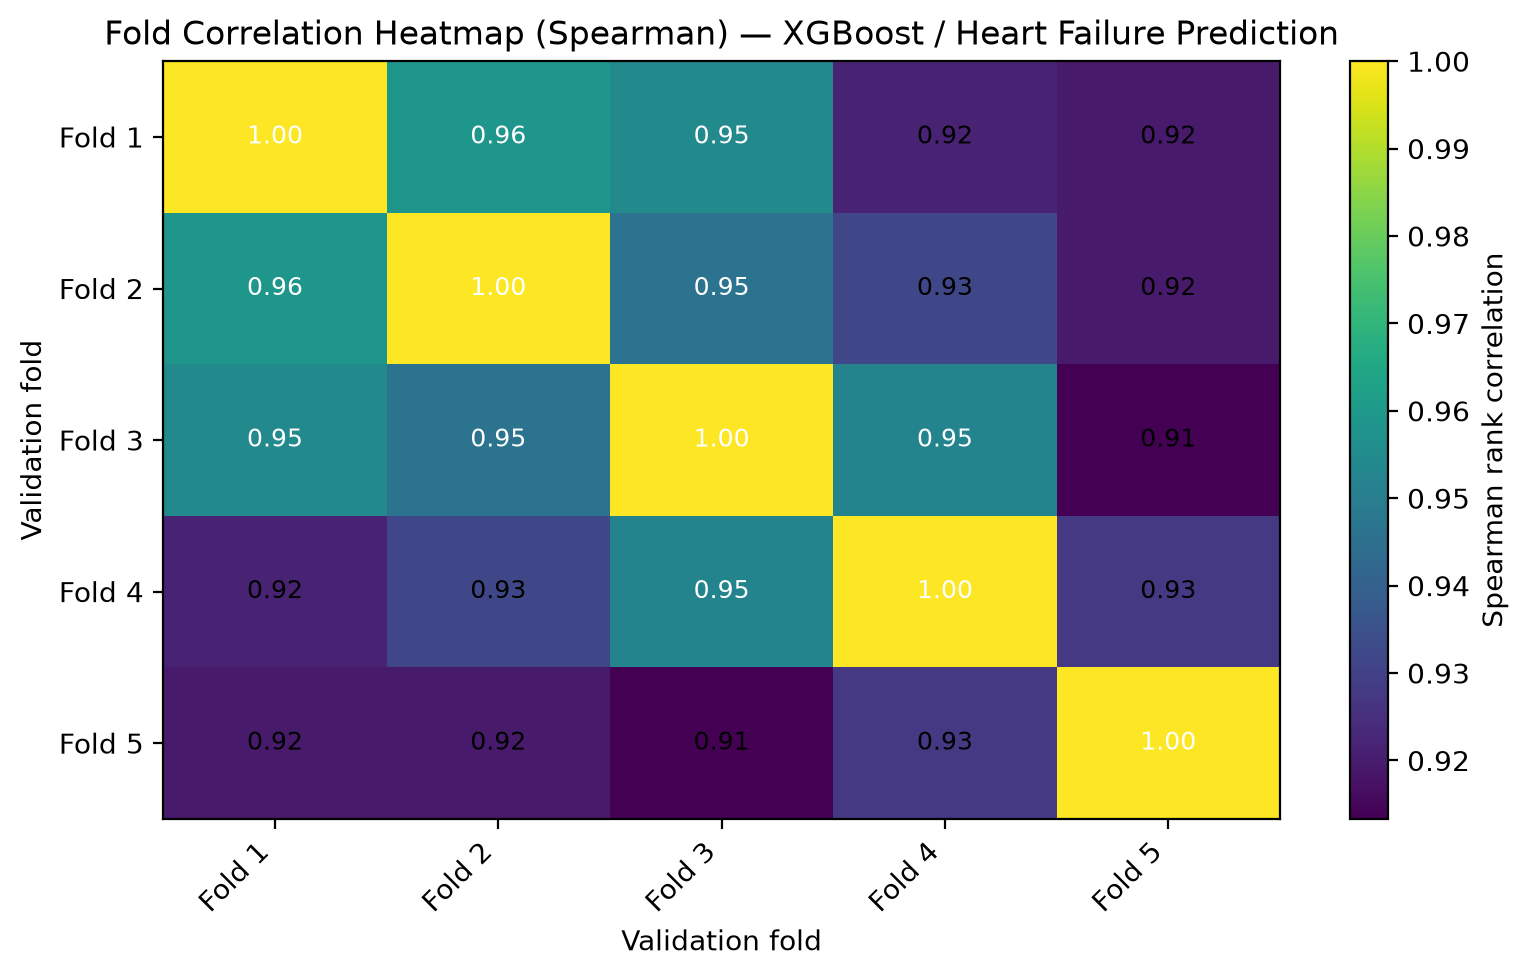
\includegraphics[width=\linewidth]{Figures/dataset2_xgboost_fold_correlation_heatmap.png}
    \end{minipage}
    \begin{minipage}{0.95\linewidth}
        \begin{figurecaptionmodern}
        \centering
        \capfig{Representative SHAP stability visualizations: feature-ranking heatmap for Dataset 1 and fold-correlation heatmap for Dataset 2 using XGBoost.}
        \label{fig:shap-stability-visualizations}
        \end{figurecaptionmodern}
    \end{minipage}
\end{figure}

The ranking heatmap makes the fold-level movement of individual features
visible, while the correlation heatmap summarizes agreement between complete
rankings. The high off-diagonal correlations in the Dataset 2 example are
consistent with its mean Spearman value of 0.9346, even though its smaller
sample produces larger predictive variability. Together, the plots clarify
that explanation stability concerns reproducibility of model rankings, not
causal importance or clinical validity.



\subsection{Discussion}

Taken together, the three research questions provide complementary evidence
about predictive quality and interpretability. RQ1 shows that XGBoost provides
the strongest overall predictive ranking across the three datasets, with
LightGBM very close on ROC-AUC and PR-AUC and AdaBoost retaining the highest
cross-dataset mean F1. RQ2 shows that predictive scores are highly stable on the
two large datasets but vary more on the smaller Heart Failure Prediction
dataset. RQ3 extends the stability analysis from prediction metrics to model
explanations and finds that the SHAP feature rankings remain highly consistent
across folds for all three boosting methods.

The SHAP results should be interpreted as measures of explanation stability,
not as evidence of causality. A feature can be consistently important to a
model because it is predictive under the observed data distribution, but this
does not establish that changing the feature would causally change a patient's
risk. In addition, raw SHAP magnitudes are not compared directly between
AdaBoost and the two gradient-boosted models because AdaBoost is explained with
permutation SHAP whereas XGBoost and LightGBM use TreeSHAP. The study therefore
bases RQ3 on within-model fold-to-fold ranking consistency, which is comparable
across the experimental protocol.

Overall, the combined findings indicate that the strongest models are not only
competitive in predictive performance but also produce feature-importance
patterns that are reproducible across data partitions. This is useful for
healthcare risk-prediction studies because an explanation that changes sharply
with a different fold would be difficult to trust even if average predictive
performance were high. The observed stability therefore provides an additional
criterion, alongside ROC-AUC, PR-AUC, Recall, and F1, for assessing the
robustness of the evaluated models.
